% Циклы с постоянным числом итераций.
% Векторизация нахождения пересечения объемной и поверхностной сеток.
\subsection{Векторизация гнезд циклов с постоянным \\ количеством итераций}\label{sec:text_4_vec_mesh_intersect}

Кроме условных операторов (\texttt{if-else}, \texttt{switch}) тело плоского цикла\label{term:flat_loop4} может содержать другие циклы и гнезда циклов.
Условия перехода на следующую итерацию и выхода из вложенного цикла также могут быть векторизованы как обычные условия \texttt{if-else}.
При этом на производительность кода влияет характер этих условий.
В этом разделе рассматривается наиболее простой случай, когда гнездо циклов, находящее в теле векторизуемого плоского цикла, выполняется с постоянным количеством итераций.

В разделе~\ref{sec:text_1_immersed_boundary_method} был описан метод погруженных границ\label{term:immersed_boundary_method2} с использованием фиктивных ячеек\label{term:cell_ibm_ghost3} для выполнения газодинамических расчетов вокруг тела со сложной геометрией.
Первым этапом его реалиазации, описанным в разделе~\ref{sec:text_1_immersed_boundary_method_realization}, является поиск пересечения всех ячеек неструктурированной поверхностной расчетной сетки\label{term:unstruct_surf_calc_mesh2} со всеми ячейками объемной декартовой сетки\label{term:mesh_descartes2}.
Для решения этой задачи требуется многократно выполнить процедуру обнаружения пересечения треугольника и прямоугольного параллелепипеда в пространстве, эта процедура описана в разделе~\ref{sec:text_1_geo_prim_tri_and_parallelepiped_int}.
Если задать координаты точек, образующих ячейки рассматриваемых расчетных сеток в виде набора массивов координат, то задачу поиска пересечений между парами ячеек (треугольник -- прямоугольный параллелепипед) можно организовать в виде плоского цикла, телом которого будет являться установление факта пересечения одной пары ячеек.
Рассмотрим подход к векторизации этого программного контекста \cite{Rybakov2019VecInt}.

\subsubsection{Оптимизация поиска пересечения расчетных сеток}

Ячейки объемной сетки являются прямоугольными параллелепипедами.
Ячейки поверхностной сетки являются треугольниками.
Для того, чтобы найти все ячейки объемной сетки, которые пересекаются с поверхностью, в общем случае необходимо проверить факт пересечения каждой объемной ячейки с каждой поверхностной ячейкой.
В общем случае данная процедура является очень затратной, так как сетки могут содержать большое количество ячеек.
Вместо этого для каждой ячейки поверхностной сетки сначала будем определять диапазон ячеек объемной сетки, с которыми в принципе возможно пересечение.

Пусть изначально объемная сетка, описывающая область $[X_l, X_h] \times [Y_l, Y_h] \times [Z_l, Z_h]$, размера $S_x \times S_y \times S_z$ разделена на одинаковые ячейки размера $s_x \times s_y \times s_z$, где
\begin{equation}
	n_x = \frac{S_x}{s_x}, \ n_y = \frac{S_y}{s_y}, \ n_z = \frac{S_z}{s_z}
\end{equation}

($n_x$, $n_y$, $n_z$ -- количество ячеек по направлению $X$, $Y$, $Z$ соответственно).

Таким образом, объемная сетка представлена трехмерным массивом ячеек, координаты которых $(x_l, x_h, y_l, y_h, z_l, z_h)$ могут быть вычислены по индексам $(i, j, k)$ в этом трехмерном массиве:
\begin{equation}
	\begin{aligned}
		& x_l(i) = X_l + i s_x, & x_h(i) = X_l + (i + 1) s_x \\
		& y_l(j) = Y_l + j s_y, & y_h(j) = Y_l + (j + 1) s_y \\
		& z_l(k) = Z_l + k s_z, & z_h(k) = Z_l + (k + 1) s_z		
	\end{aligned}
\end{equation}

Для треугольника, являющегося ячейкой поверхностной сетки, вершинами которого являются точки $A$, $B$, $C$, можно найти охватывающий прямоугольный параллелепипед, координаты которого равны

\begin{equation}
	\begin{aligned}
		& \tilde{x}_l = \min(x_A, x_B, x_C), & \tilde{x}_h = \max(x_A, x_B, x_C) \\
		& \tilde{y}_l = \min(y_A, y_B, y_C), & \tilde{y}_h = \max(y_A, y_B, y_C) \\
		& \tilde{z}_l = \min(z_A, z_B, z_C), & \tilde{z}_h = \max(z_A, z_B, z_C)
	\end{aligned}
\end{equation}

Если треугольник пересекает некоторую объемную ячейку, то его охватывающий прямоугольный параллелепипед также пересекает эту ячейку.
То есть для определения пересечения поверхностной ячейки со всеми ячейками объемной сетки достаточно проверить только те ячейки, с которыми пересекается охватывающий прямоугольный параллелепипед рассматриваемого треугольника.
Так как координаты анализируемых параллелепипедов могут быть записаны явно, то можно вычислить диапазоны индексов ячеек, которые требуется проверить на предмет пересечения с треугольником.
Факт пересечения по координате $x$ двух отрезков $[x_l(i), x_h(i)]$ и $[\tilde{x}_l, \tilde{x}_h]$ можно записать в виде системы из двух неравенств
\begin{equation}\label{eqn:text_4_mesh_intersect_eq2}
	\left\{
		\begin{aligned}
			x_l(i) \le \tilde{x}_h \\
			x_h(i) \ge \tilde{x}_l
		\end{aligned}
	\right.
\end{equation}

Преобразовав систему \eqref{eqn:text_4_mesh_intersect_eq2}, и выполнив аналогичные действия для координат по $y$ и $z$, получим диапазоны индексов ячеек объемной сетки
\begin{equation}\label{eqn:text_4_mesh_intersect_diap}
	\left\{
		\begin{aligned}
			\frac{\tilde{x}_l - X_l}{s_x} - 1 \le i \le \frac{\tilde{x}_h - X_l}{s_x} \\
			\frac{\tilde{y}_l - Y_l}{s_y} - 1 \le j \le \frac{\tilde{y}_h - Y_l}{s_y} \\
			\frac{\tilde{z}_l - Z_l}{s_z} - 1 \le k \le \frac{\tilde{z}_h - Z_l}{s_z}
		\end{aligned}
	\right.
\end{equation}

Диапазон индексов из \eqref{eqn:text_4_mesh_intersect_diap} содержит малую долю всех ячеек объемной сетки.
В этом случае не требуется проводить анализ ускорения от этого преобразования, так как при его отсутствии поиск пересечения сеток просто нежизнеспособен.

\subsubsection{Векторизация пересечения пар ячеек}

Рассмотрим реализацию функции \texttt{tri\_box\_intersect}, анализирующую наличие пересечения треугольника и прямоугольного параллелепипеда с помощью метода свертывания системы линейных неравенств\label{term:method_svert_sys_neravenstv2} из \cite{Chernikov1963} (см. листинг~\ref{lst:text_1_mesh_intersect_tri}).

\begin{singlespace}
\begin{lstlisting}[caption={Исходная реализация свертывания системы линейных неравенств для определения пересечения треугольника и прямоугольного параллелепипеда.},label={lst:text_1_mesh_intersect_tri}]
for (i = 0; i < bec; ++i)
{
    gi0 = g[i][0];

    if (gi0 == 0.0)
    {
        if (!upgrade(g[i][1], g[i][2], &lo, &hi))
        {
            return 0;
        }
    }
    else
    {
        for (j = i + 1; j < bec; ++j)
        {
            if (gi0 * g[j][0] < 0.0)
            {
                f0 = gi0 * g[j][1] - g[j][0] * g[i][1];
                f1 = gi0 * g[j][2] - g[j][0] * g[i][2];

                if (gi0 < 0.0)
                {
                    f0 = -f0;
                    f1 = -f1;
                }

                if (!upgrade(f0, f1, &lo, &hi))
                {
                    return 0;
                }
            }
        }
    }
}

return 1;
\end{lstlisting}
\end{singlespace}

Функция возвращает $1$, если пересечение есть, и $0$, если пересечения нет.
Логика работы функции следующая.
Сначала коэффициенты системы неравенств \eqref{eqn:text_1_geo_prim_2} заносятся в двумерный массив коэффициентов \texttt{g[bec][3]}, где \texttt{bec} (basic equations count) -- количество исходных неравенств системы (в нашем случае 9).
Затем выполняется один шаг деформации системы\label{term:deform_sys_lin_neravenstv2} с одновременным поиском множества решения для переменной $\gamma$.
Перед началом свертывания множество допустимых значений для переменной $\gamma$ принимается в виде отрезка $[0, 1]$ (\texttt{lo = 0}, \texttt{hi = 1}).
По мере свертывания системы неравенств \eqref{eqn:text_1_geo_prim_2} происходит сокращение множеств решений.
Если на каком-то этапе свертывания множество решений обращается в пустое (\texttt{lo > hi}), то функция заканчивает работу и возвращает 0.
Если после выполнения всех действий свертывания множество решений осталось ненулевым, то это означает наличие пересечения, и функция возвращает 1.

Получившийся программный код можно охарактеризовать как имеющий сложное управление, уровень вложенности конструкций управления в нем достигает 5 (\texttt{for-if-for-if-if}), к тому же участок содержит 3 выхода из функции.
Функция \texttt{upgrade}, которая вызывается в строке 7 листинга, предназначена для обновления текущего множества допустимых значений для переменной $\gamma$ с учетом нового полученного ограничения вида $k_{\gamma} \gamma + k \le 0$, коэффициенты которого передаются в первом и втором параметрах.
Текущее множество решений является отрезком с границами, хранящимися в переменных \texttt{lo} и \texttt{hi}, и в зависимости от знака коэффициента $k_{\gamma}$ одна из этих границ внутри вызова функции \texttt{upgrade} может измениться (граница \texttt{lo} может увеличиться, либо граница \texttt{hi} может уменьшиться).
Если после обновления множества решений оно оказывается пустым (нижняя граница становится больше верхней), то функция \texttt{upgrade} возвращает 0, в противном случае она возвращает 1.

После рассмотрения реализации функции \texttt{tri\_box\_intersect} можно перейти к векторизации вычислений\label{term:vectorization3}.
Для анализа пересечения двух сеток необходимо вызывать функцию \texttt{tri\_box\_intersect} многократно с разными наборами входных параметров.
Для оптимизации этого процесса реализуем функцию \texttt{tri\_box\_intersect\_16}, объединяющую внутри себя обработку 16 вызовов функции \texttt{tri\_box\_intersect} (используется объединение 16 вызовов, так как это совпадает с количеством элементов вещественных данных одинарной точности в одном zmm регистре).
В первом приближении реализация функции \texttt{tri\_box\_intersect\_16} представлена на листинге~\ref{lst:text_1_mesh_intersect_tri16}.

\begin{singlespace}
\begin{lstlisting}[caption={Исходная реализация функции, объединяющей 16 вызовов функции \texttt{tri\_box\_intersect}.},label={lst:text_1_mesh_intersect_tri16}]
void tri_box_intersect_16(float* xa, float* ya, float* za,
                          float* xb, float* yb, float* zb,
                          float* xc, float* yc, float* zc,
                          float* xl, float* xh,
                          float* yl, float* yh,
                          float* zl, float* zh,
                          int* r)
{
  for (int i = 0; i < w; ++i)
  {
    r[i] = tri_box_intersect(xa[i], ya[i], za[i],
                             xb[i], yb[i], zb[i],
                             xc[i], yc[i], zc[i],
                             xl[i], xh[i], yl[i], yh[i], zl[i], zh[i]);
  }
}
\end{lstlisting}
\end{singlespace}

Для векторизации функции \texttt{tri\_box\_intersect\_16} следует выполнить подстановку тела функции \texttt{tri\_box\_intersect} в место ее вызова.
После выполнения этого преобразования получаем программный контекст, содержащий сложное управление, частности гнездо из трех вложенных циклов, не считая условий.
Такой контекст не может быть векторизован компилятором автоматически, поэтому будем проводить его векторизацию в ручном режиме с использованием функций-интринсиков\label{term:intrinsic4}.

Заметим, что между итерациями внешнего цикла (листинг~\ref{lst:text_1_mesh_intersect_tri16}, строка 9) отсутствуют зависимости, то есть цикл является плоским, и его итерации могут быть выполнены в любом порядке, в том числе и одновременно.
Такие циклы поддаются векторизации путем перевода тела в предикатное представление\label{term:predicate_view2} и заменой скалярных инструкций на векторные.
Наиболее тонким местом при векторизации тела плоского цикла являются условия, то есть наличие конструкций \texttt{if-else}.
Альтернативные ветви таких конструкций должны быть объединены в предикатном коде под противоположными предикатами.
Наличие большого количества условных операторов в исходном коде порождает множество инструкций под нулевыми предикатами в результирующем коде, что негативно сказывается на производительности.
Для уменьшения количества условных операторов, можно использовать математические тождества, заменяющие условные конструкции на команды, имеющие векторные аналоги в наборе инструкций AVX-512\label{abbr:avx6}.
Для этих целей хорошо подходят такие векторные команды как abs, min, max, blend и другие.
Например, в рассматриваемом коде вычисление значений \texttt{f0} и \texttt{f1} в строках 18-25 на листинге~\ref{lst:text_1_mesh_intersect_tri} с учетом условия \texttt{g[i][0] * g[j][0] < 0} может быть заменено на следующее:

\begin{singlespace}
\begin{lstlisting}[caption={Использование тождества для векторизации условия.},label={lst:text_4_mesh_intersect_tozh}]
f0 = fabs(gi0) * g[j][1] + fabs(g[j][0]) * g[i][1]
f1 = fabs(gi0) * g[j][2] + fabs(g[j][0]) * g[i][2]
\end{lstlisting}
\end{singlespace}

Похожие трудности вызывает условие \texttt{if} в строке 5 на листинге~\ref{lst:text_1_mesh_intersect_tri}.
Это условие имеет альтернативную ветку, содержащую цикл.
Слияние этих двух ветвей снижает производительность результирующего кода, поэтому в этом случае выгодно применить расщепление внешнего цикла по условию\label{term:loop_split_by_cond3} (по конструкции \texttt{if-else}).
При этом образуются два гнезда циклов, каждое из которых может быть векторизовано независимо.
Заметим, что описанное преобразование в общем смысле не является эквивалентным, так как обе ветки условия \texttt{if-else}, а значит и тела образовавшихся циклов, содержат выходы из функции, выполнение расщепления цикла может изменить условие, провоцирующее выход из функции.
По этой причине компилятор не способен выполнить такое преобразование автоматически.
Однако с точки зрения результата функции описанное преобразование корректно, поэтому мы его и применяем.

Отметим еще один крайне положительный момент в рассматриваемом программном контексте.
Условием выхода из вложенных циклов является достижение индуктивной переменной значения \texttt{bec}.
Это значение является константой, а значит не зависит от номера итерации, поэтому в векторный код это условие может быть перенесено без изменений.
В случае зависимости условия выхода из цикла от номера итерации само условие должно быть также векторизовано, что может привести к потерям производительности.
Однако в рассматриваемом коде проблем векторизации циклов с непостоянным количеством итераций нет.
На рис.~\ref{fig:text_1_mesh_intersect_scheme} приведен получившийся предикатный код для функции \texttt{tri\_box\_intersect\_16}, а также схематично показана его транформации в векторный аналог.

\begin{figure}[ht]
\centering
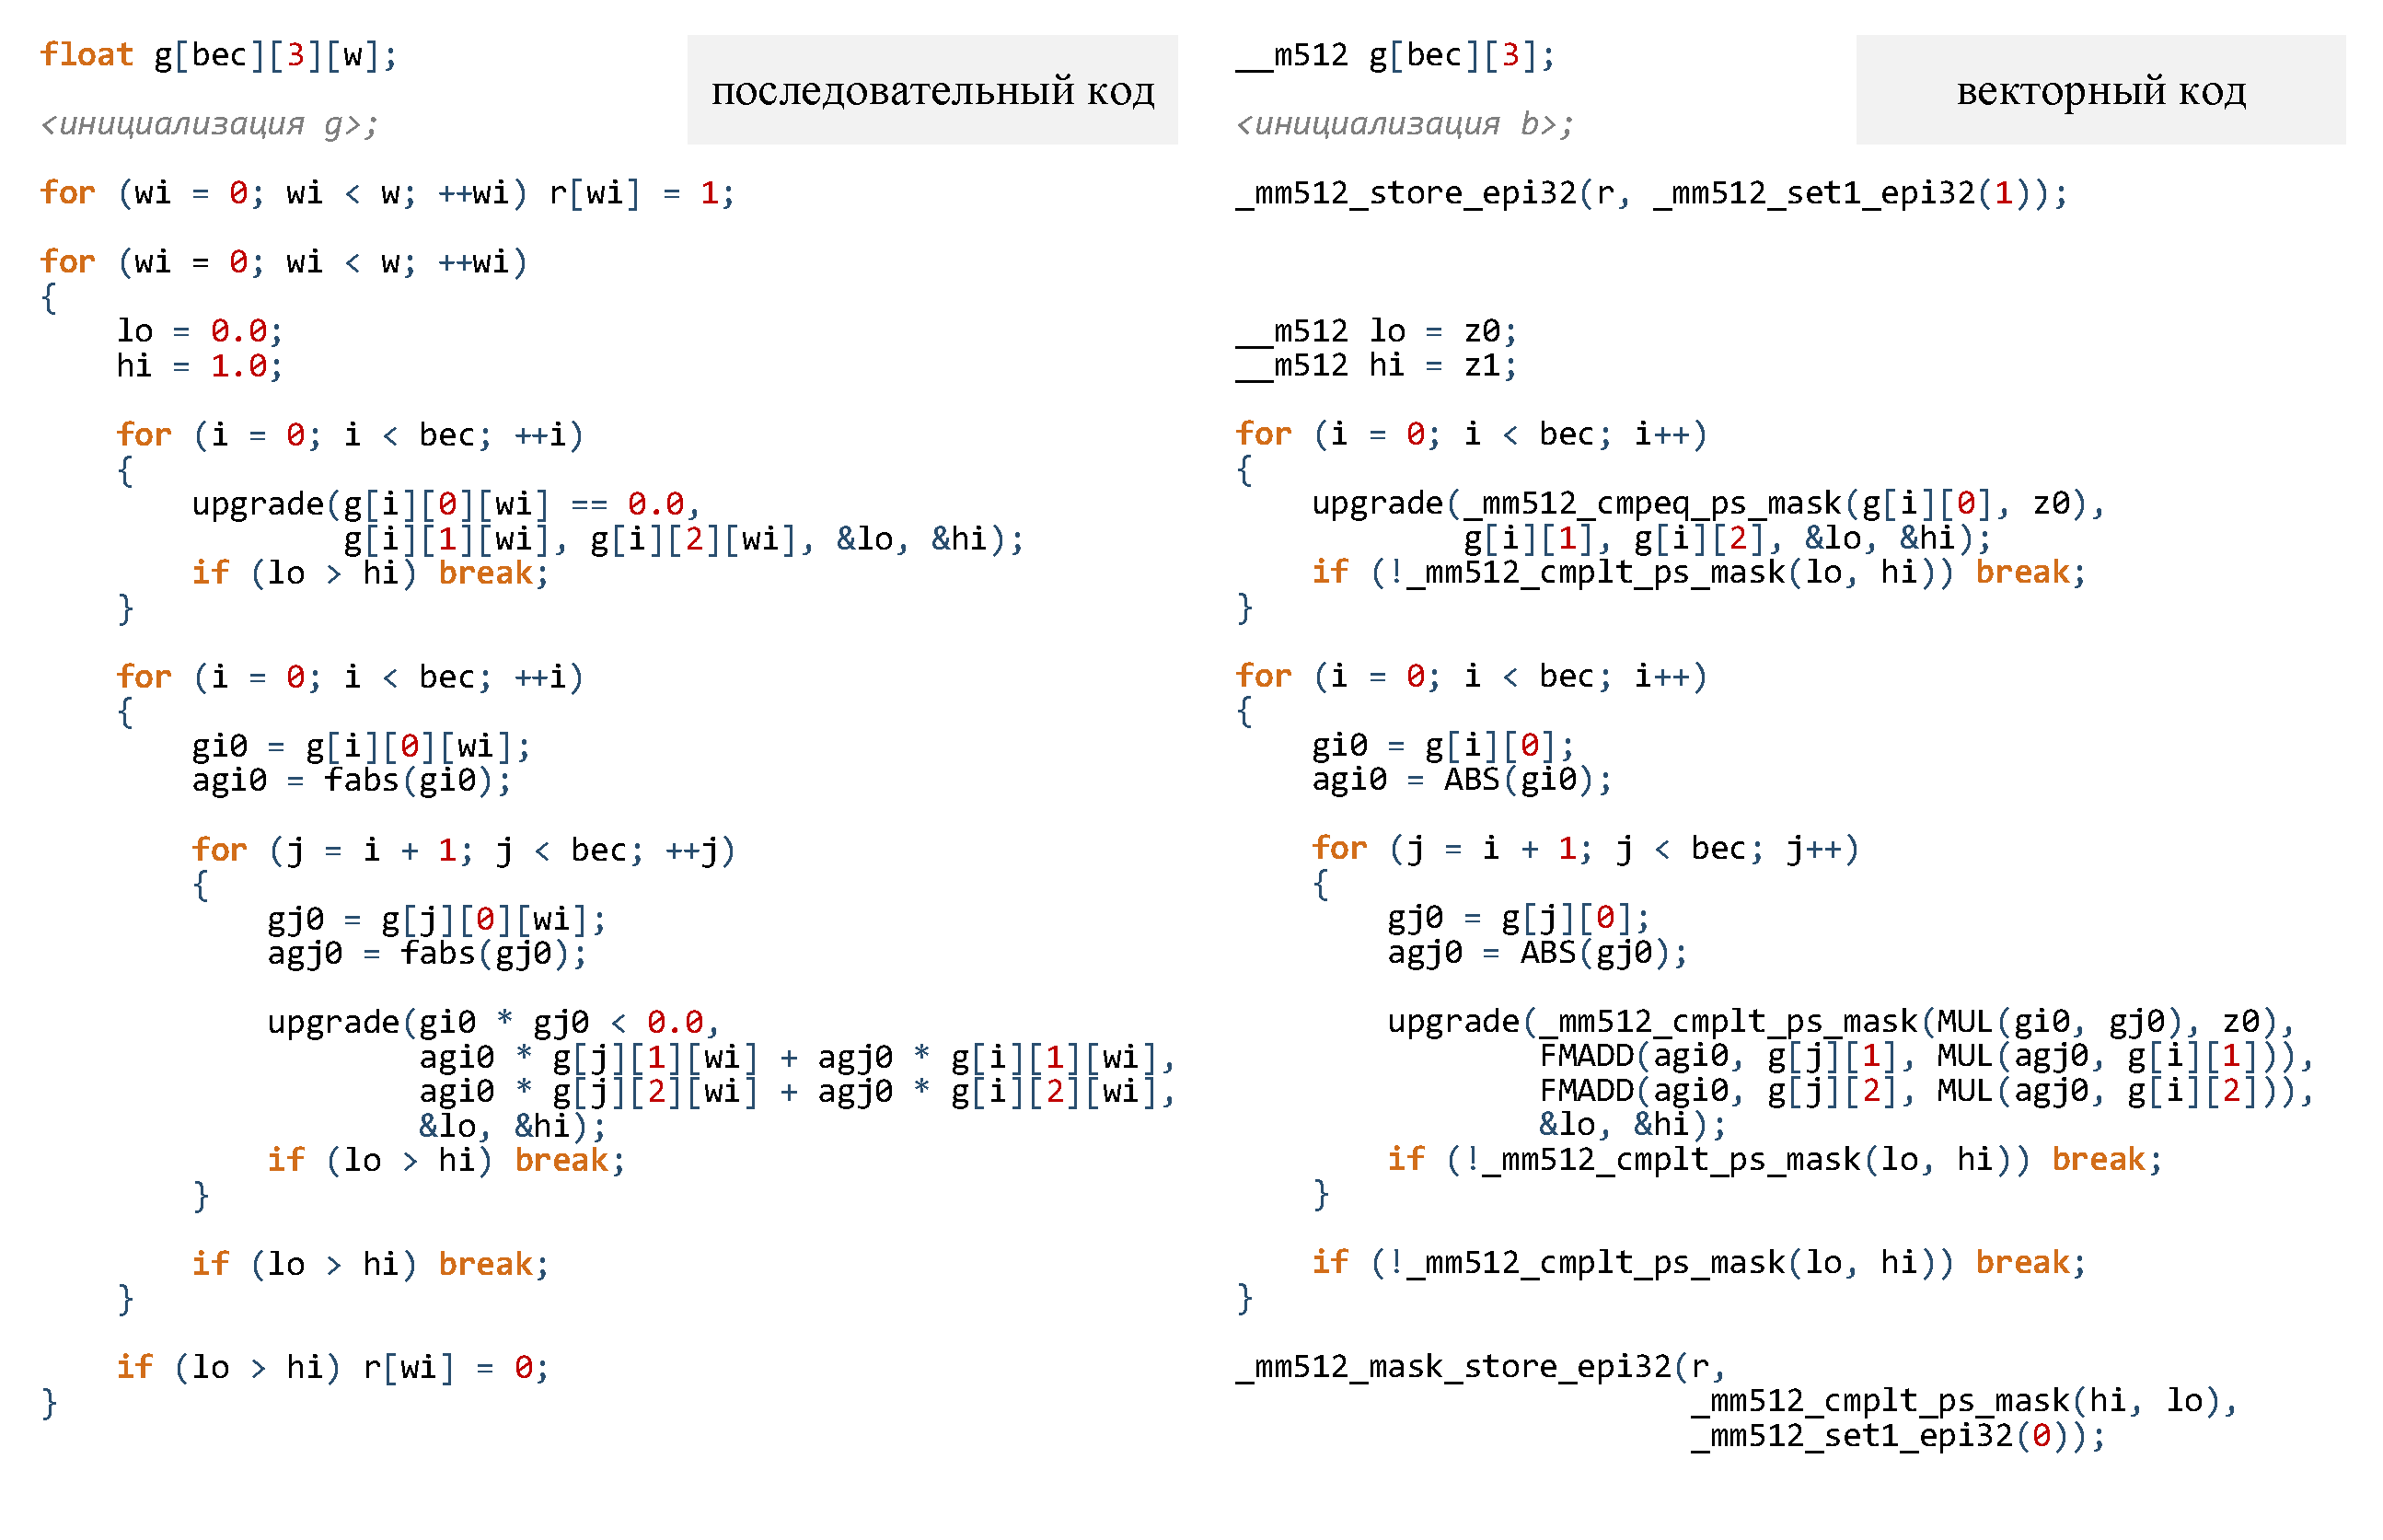
\includegraphics[width=1.0\textwidth]{./pics/text_4_mesh_intersect/final_scheme.pdf}
\singlespacing
\captionstyle{center}\caption{Схема перевода последовательного кода в векторный аналог для ядра функции \texttt{tri\_box\_intersect\_16}.}
\label{fig:text_1_mesh_intersect_scheme}
\end{figure}

Из рис.~\ref{fig:text_1_mesh_intersect_scheme} видно, что правильно составленный предикатный код (на рисунке слева) может быть довольно просто переведен в векторный аналог.
Для этого должны соблюдаться некоторые простые требования.
Во-первых, необходимо удалить все \texttt{else} ветки в условных операторах.
Этого можно добиться, например, путем расщепления оператора \texttt{if-else} на два противоположных условия.
После этого любое условие \texttt{if} легко трансформируется в предикат на весь блок кода, находящийся под условием.
Во-вторых, вызовы функции не должны находиться под предикатами.
Вместо этого в нашем случае скалярное условие вызова функции \texttt{upgrade} трансформировалось в аргумент функции, и после этого код легко поддается векторизации.
В остальном все вещественные скалярные инструкции были просто заменены на векторные аналоги.
Также была выполнена векторизация функции \texttt{upgrade} с помощью слияния всех веток выполнения под их предикатами\label{term:meth_vec_merge2}, результирующий код этой функции представлен на листинге~\ref{lst:text_4_mesh_intersect_upgrade}.

\begin{singlespace}
\begin{lstlisting}[caption={Векторная реализация функции upgrade с пропагированным условием вызова внутрь функции.},label={lst:text_4_mesh_intersect_upgrade}]
void upgrade(__mmask16 m, __m512 f0, __m512 f1,
             __m512 *lo, __m512 *hi)
{
    __mmask16 c_f0z = _mm512_cmpeq_ps_mask(f0, z0);
    __mmask16 c_f0n = _mm512_cmplt_ps_mask(f0, z0);
    __mmask16 c_f0p = ~(c_f0z | c_f0n);
    __mmask16 c_f1p = _mm512_cmplt_ps_mask(z0, f1);
    __m512 k = _mm512_mask_div_ps(k, ~(m & c_f0z), f1, f0);
    k = SUB(z0, k);
    *lo = _mm512_mask_add_ps(*lo, m & c_f0z & c_f1p, *hi, z1);
    *hi = _mm512_mask_min_ps(*hi, m & c_f0p, *hi, k);
    *lo = _mm512_mask_max_ps(*lo, m & c_f0n, *lo, k);
}
\end{lstlisting}
\end{singlespace}

В результате выполненных преобразований был получен достаточно эффективный векторный код для поиска пересечений поверхностной и объемной расчетных сеток.
Функция определения пересечения пар ячеек (треугольник -- прямоугольный параллелепипед) продемонстрировала ускорение в 6,7 раза по сравнению с невекторизованной версией на микропроцессоре Intel Xeon Phi 7290 KNL\label{abbr:knl12}.
Полные версии программного кода, приведенного в разделе, доступны в \cite{iparGithub}.
